\documentclass[../NFTComp_IEEE.tex]{subfiles}
\graphicspath{{\subfix{../Images}}}

\begin{document}
\section{Development of a NFT Smart Contract in Cadence}
\label{sec:cadence_development}
The central exercise of this paper begun with the development of a Cadence NFT smart contract following Flow's standard for non-fungible tokens. The idea is to keep this process as close as possible to its homologue in Ethereum. As such, the Cadence implementation was kept to as simple as possible to ensure the comparison to focus on the maximum of common elements to both architectures as possible. Fig. \ref{fig:cadence_nft_contract} presents a schematic representation of the contract developed displaying the required standard dependencies and the functions and parameters imposed by their inheritance.

\begin{figure}[h!]
    \centering
    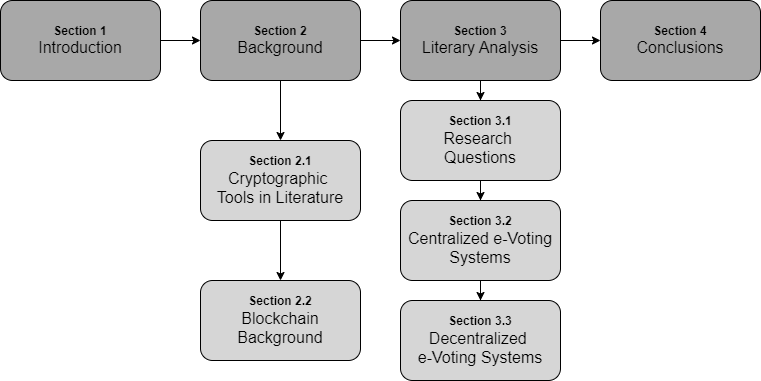
\includegraphics[width=\columnwidth]{Images/almei1.png}
    \caption{Structural organisation of a NFT smart contract in Cadence}
    \label{fig:cadence_nft_contract}
\end{figure}

\subsubsection{Standards Imported}
The simplest standardised version of a Cadence NFT smart contracts requires the import of two standards, namely, \textit{NonFungibleToken} and \textit{MetadataViews} interfaces. We omitted references to the \textit{MetadataViews} because this standard does not has a corresponding standard in Ethereum. Flow was developed to support digital collectible projects, which emulate real world collectible systems, like trading cards for example. This emphasises the metadata operations associated to the NFTs produced, hence why Cadence produced a standard to deal specifically with NFT metadata operations. There's a dependence between the \textit{NonFungibleToken} standard and \textit{MetadataViews}, hence why a basic NFT contract has to import both, but the \textit{MetadataViews} requirements are minimal and are not consequential to this comparison.
\par
We used a color scheme in Fig. \ref{fig:cadence_nft_contract} to indicate which standard required the implementation of the function, resources and events indicated in the contract. The \textit{MetadataViews} requirement imposes the implementation of a pair of functions used to set and retrieve metadata related items in the contract. These functions were implemented but are "empty" in the sense that they simply return an empty element of the value defined as return to minimise their influence in the contract.

\paragraph{Resources}
Only the \textit{NonFungibleToken} standard imposes the implementation of a NFT and a collection resources, the latter used to ease the storage of multiple resources, as it was mentioned in Sec. \ref{sec:resource_collections}. A NFT and a Collection definition are the minimal requirements from Flow in this regard. But Fig. \ref{fig:cadence_nft_contract} indicates a third resource included in the contract, namely a \textit{NFTMinter}. This resource is used to abstract, simplify and secure the minting of new NFTs from this contract. A NFT minter is not required by any of the standards, but the contract becomes unusable without one, so it is a sort of implicit requirement. This happens because new resources can only be created with a contract function due to Cadence restricting the use of the "\textbf{create}" keyword to the context of the contract and within a function. Transactions are not able to invoke this internal action. A secure approach to create new NFT resources is to define the function that creates new ones inside of a NFT minter resource and having this minter resource created and saved into the contract deployer storage in the contract constructor. This restricts the creation of new NFTs to the owner of the storage space where the minter was saved, i.e., the contract deployer, while making it impossible to create new NFTs from the contract itself, thus decoupling this action from the contract itself.

\paragraph{Functions}
The \textit{NonFungibleToken} standard requires the implementation of a \textit{createEmptyCollection} function to obtain a collection resource. Unlike NFTs, this contract provides multiple access points to create new collections. The \textit{NonFungibleToken} standard also imposes a similar function in the NFT resource definition and the collection resource itself. This may sound redundant, but in standardised NFT contracts in Flow allow collections to create other collections. The \textit{createEmptyCollection} function in Fig. \ref{fig:cadence_nft_contract} requires a type as input because it is not possible to infer the type of any resource to store at the contract level, therefore this needs to be provided. The versions of this function implemented in the NFT and collection resources do not need it because they can infer the type to store from the resource itself.

\paragraph{Events}
A contract that imports the \textit{NonFungibleToken} inherits the \textit{Withdrawn} and \textit{Deposited} events by default. In Cadence, like in Solidity, events are made available and emitted automatically by the logic imported from the standards, i.e., there is no need to define them explicitly in the contracts, unlike functions and resources. The events indicated are emitted automatically whenever a NFT resource is moved in or out of an account storage.

\end{document}